\subsection{第 9 课 | DFS 和 BFS}

\subsubsection{脑图}

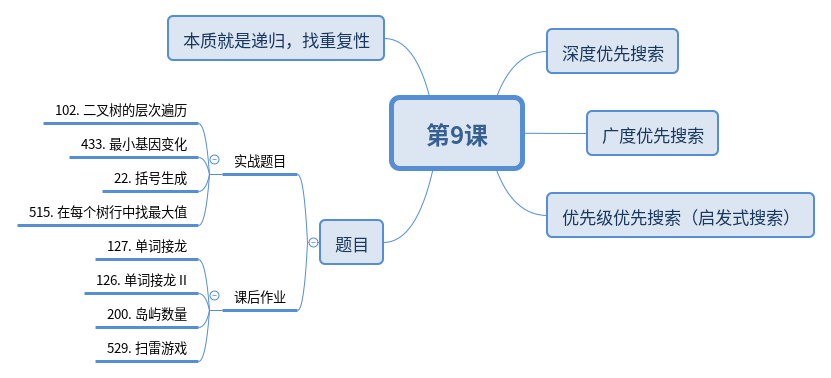
\includegraphics[width=170mm,height=80mm]{images/第9课.png}

\subsubsection{题目}

\paragraph{实战题目}

\begin{itemize}
  \item \hyperref[leetcode:102]{102. 二叉树的层次遍历}
  \item \hyperref[leetcode:433]{433. 最小基因变化}
  \item \hyperref[leetcode:22]{22. 括号生成}
  \item \hyperref[leetcode:515]{515. 在每个树行中找最大值}
\end{itemize}

\paragraph{课后作业}

\begin{itemize}
  \item \hyperref[leetcode:127]{127. 单词接龙}
  \item \hyperref[leetcode:126]{126. 单词接龙 II}
  \item \hyperref[leetcode:200]{200. 岛屿数量}
  \item \hyperref[leetcode:529]{529. 扫雷游戏}
\end{itemize}
